\clearpage
\twocolumn[{%
\rqparent
\subsection{Decision accuracy against a no-signal null}
\label{app:rq02_permutation_null}

\noindent\begin{minipage}[t]{0.485\textwidth}
\vspace{0pt}
\paragraph{Research Question.} \emph{How far above chance does a proxy rank the design decisions, once chance is measured cell by cell rather than read off a flat 0.5?}

\paragraph{Setup.} We measure how far DA-size lies above the agreement that a proxy without signal reaches in the same cell. We use the seed-1904 runs of every language setting, ladder and data build. The proxies (90M--1B) are compared against the final 1.7B checkpoint, on pairs that differ on any number of design axes. The tasks are the benchmark tasks above chance at the proxy and at 1.7B, the bBPB twins included, and the per-language BPB of the 50 trained languages. A (task, proxy size) cell needs three comparable pairs. We shuffle the proxy's final scores across the design variants 1000 times. Each shuffle is scored against the unchanged 1.7B ranking with the same sign rule, ties included. A cell's p-value is the share of shuffles that match at least as many pairs as the real proxy, corrected over the cells with the Benjamini-Hochberg procedure. Each pooled line divides the matching pairs by the comparable pairs, summed over cells, and its band is the 95 \% range of the pooled shuffles.
\end{minipage}\hfill
\begin{minipage}[t]{0.485\textwidth}
\vspace{0pt}
\begin{rqfinding}
\textbf{1. The benchmark null sits below 0.5.} Pooled over the benchmark tasks, a shuffled proxy scores 0.49 because proxy ties count as misses, so the observed 0.57--0.59 lies 0.08--0.10 above its null rather than 0.07--0.09 above 0.5. (Figure~\ref{fig:app_rq02_permutation_null}.)
\\
\\
\textbf{2. Few benchmark cells beat their own null.} Only 8--10 \% of the multi-axis benchmark cells (0--2 \% of the mono-axis ones) are above their null at q $<$ 0.05, so the pooled lines clear the null because many weak cells add up, not because single tasks rank the decisions.
\\
\\
\textbf{3. BPB is far above its null.} Per-language BPB reaches 0.78--0.94 against a null of 0.50, and 30--64 \% of its multi-axis cells are significant (4--40 \% mono-axis, where a cell has fewer pairs).
\end{rqfinding}
\end{minipage}

\vspace{\baselineskip}
\noindent\begin{minipage}{\textwidth}
\centering
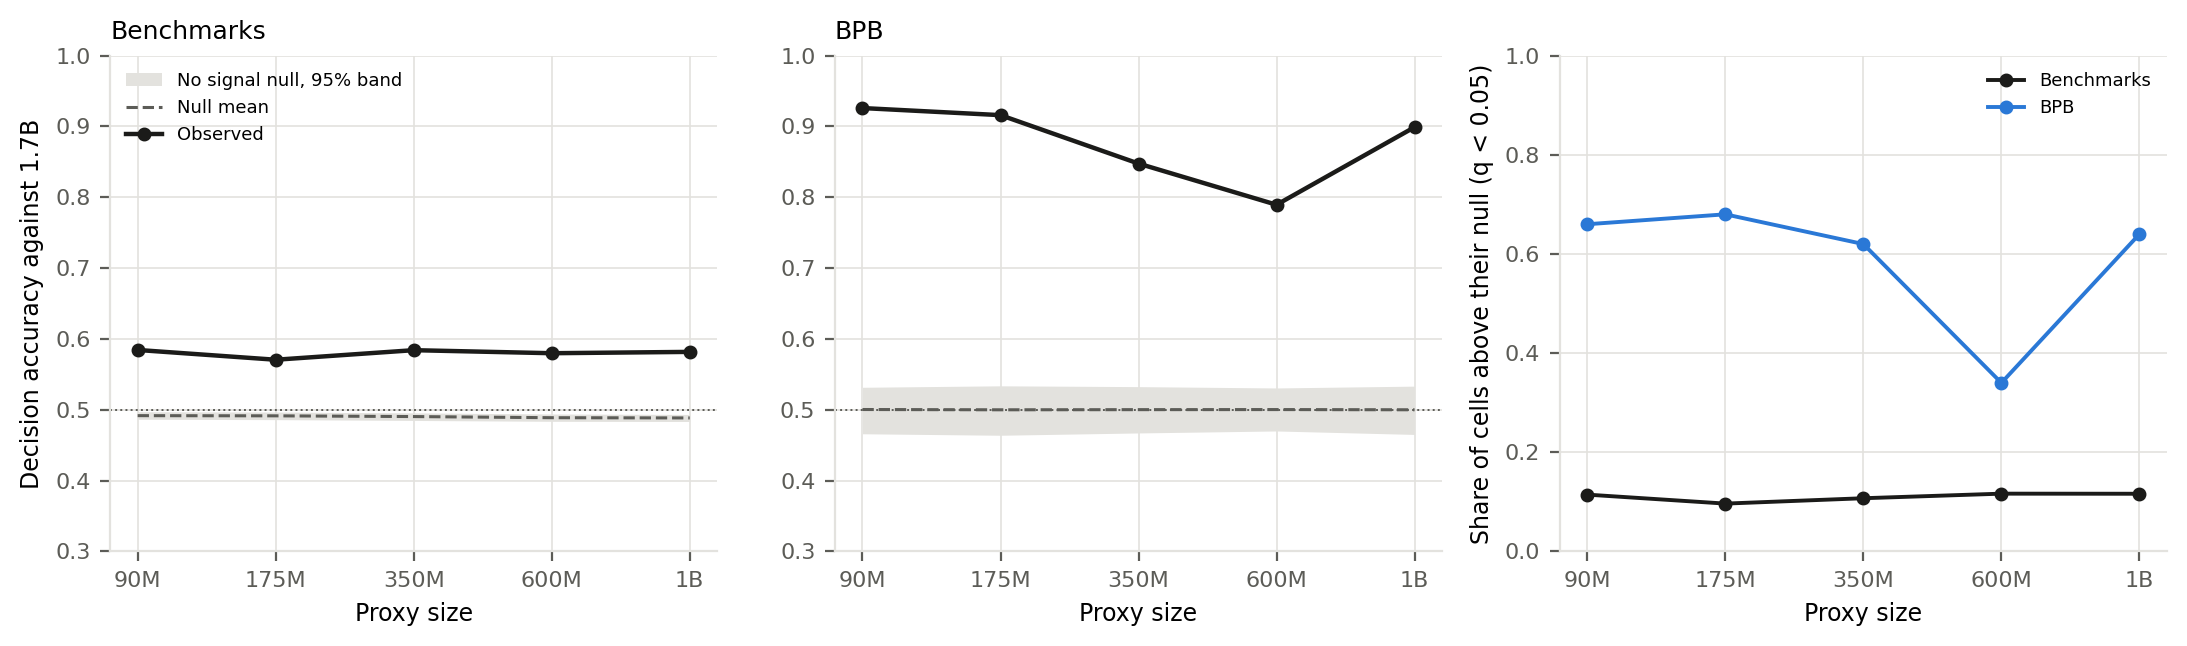
\includegraphics[width=\textwidth,height=0.36\textheight,keepaspectratio]{figures/app_rq02_permutation_null.png}
% source: src/signal-and-noise/analysis/rq02_permutation_null/pretraining/predictivity/permutation_null_da_size_paper.png
\captionof{figure}{\textbf{The benchmark null sits below 0.5.} DA-size of the final checkpoint of each proxy size against the 1.7B final checkpoint, on multi-axis design pairs, pooled over decisions, for the benchmark tasks with their bBPB twins (left) and the per-language bits per byte (middle). The black line is the observed DA-size, the dashed grey line the mean of the shuffled null and the grey band its 95\% range. The dotted line marks 0.5. Right: the share of (task, proxy size) cells above their own null at q $<$ 0.05.}
\label{fig:app_rq02_permutation_null}
\end{minipage}
}]
